% LaTeX Template for Project Report, Version 2.0
% Released under Creative Commons Attribution license (CC-BY)
% Info: http://creativecommons.org/licenses/by/3.0/
%
% It is advisable to learn the basics of LaTeX before using this template.
% A good resource to start with is http://en.wikibooks.org/wiki/LaTeX/
%
% Empty space after chapter/section/subsection titles can be used to insert text.
%
% Just compile this file using pdflatex after making all required changes.
\documentclass[12pt,a4paper]{report}
\usepackage[pdftex]{graphicx} %for embedding images
\usepackage{tabularx}
\usepackage{multirow}
\usepackage{subcaption}
\usepackage{placeins}
\usepackage{url} %for proper url entries
\usepackage[backend=biber]{biblatex}
\bibliography{ref.bib}


\begin{document}
\renewcommand\bibname{References} %Renames "Bibliography" to "References" on ref page

%include other pages
\begin{titlepage}
\clearpage
\thispagestyle{empty}
\begin{center}

\textup{\large{  \bf CSD334 Mini Project Report }}\\[0.2in]

% Title
\Large \textbf {Project Management System}\\[0.5in]

       \small \emph{Submitted in partial fulfillment of\\
        the requirements for the award of the degree of}
        \vspace{.2in}

       {\bf Bachelor of Technology \\in\\ Computer Science and Engineering}\\[0.5in]

% Submitted by
\normalsize Submitted by \\
\begin{table}[h]
\centering
\begin{tabular}{lr}\hline \\
Register No. & Name of Student \\ \\ \hline
\\
KNR19CS003  & Abhiram Rajeevan \\
KNR19CS024  & Aswin V Nair \\ 
KNR19CS029  & Jithesh Raj M  \\ 
KNR19CS040  & Muhammed Naseef M P \\ \\ \hline 
\end{tabular}
\end{table}

\vspace{.1in}
Under the guidance of\\
{\textbf{Dr. Dileep M R}}\\[0.2in]

\vfill

% Bottom of the page

\includegraphics[width=0.18\textwidth]{./gcek_logo.jpg}\\[0.1in]
\Large{Department of Computer Science and Engineering}\\
\normalsize
\textsc{Government College of Engineering Kannur}\\
Kannur, Kerala State, India -- 670563 \\
\vspace{0.2cm}


\end{center}

\end{titlepage}

\newpage
\thispagestyle{empty}

\begin{center}

\huge{Department of Computer Science and Engineering}\\[0.5cm]
\normalsize
\textsc{Government College of Engineering Kannur}\\[2.0cm]

\emph{\LARGE Certificate}\\[1.0cm]
\end{center}

\normalsize This is to certify that this is a bonafide record of the Mini Project work 
done by the student whose name is given below in partial fulfillment of the requirements of the 
degree of Bachelor of Technology in Computer Science and Engineering under A.P.J.Abdul Kalam Technological 
University during the year 2022-23.\\[1.0cm]

\begin{table}[h]
\centering
\begin{tabular}{lr}
Register No. & Name of Student \\ \\ \hline
\\
KNR19CS003  & Abhiram Rajeevan \\  
KNR19CS024  & Aswin V Nair \\ 
KNR19CS029  & Jithesh Raj M  \\ 
KNR19CS040  & Muhammed Naseef M P \\ \\
%Enter the roll no and name of a particular team member here
\end{tabular}
\end{table}


\begin{table}[h]
\centering
\begin{tabular}{ccc}
Prof. Dileep M R & Prof. Sajith B. & Dr. Rafeeque P. C.\\
 (Project Guide) & (Project Coordinator) & (Professor and H.o.D)\\
\end{tabular}
\end{table}

% Bottom of the page






\clearpage
\vspace{1.0in}
\begin{center} 
\section*{Institute Vision}
\begin{flushleft}
``A globally renowned institution of excellence in engineering, 
 education, research and consultancy.''
\end{flushleft}

\section*{Institute Mission}
\begin{flushleft}
``To contribute to the society by providing quality education and training, leading to innovation, 
entrepreneurship and sustainable growth.''
\end{flushleft}

\section*{Department Vision}
\begin{flushleft}
``To be a centre of excellence in the field of Computer Science \& Engineering education and 
research, which extends its appreciated services to the industry and the society.''
\end{flushleft}

\section*{Department Mission}
\begin{flushleft}
``To develop engineers with excellent analytic, design and implementation skills, who can 
expertise themselves as computer professionals, research engineers, entrepreneurs or as managers, 
while fulfilling their ethical and social responsibilities, in a globally competitive environment.''
\end{flushleft}
\end{center}



\pagenumbering{roman} %numbering before main content starts
\setcounter{page}{0}

\chapter*{Acknowledgements}

We  would like to express our profound gratitude and thanks to our project
guide Dr. Dileep M R, for introducing the present topic and intellectual support , inspiring guidance and his invaluable encouragement, suggestions and cooperation helps a lot to completion of the project work successfully. We are also thankful to Prof. Sajith B. for providing necessary information and guidance regarding the project. Last but not the least, We would like to thank
our friends and family for the support and encouragement they have given
us during the course of our work.




 

\addcontentsline{toc}{chapter}{Acknowledgements}

\chapter*{Abstract}
Project management involves planning, organizing, and managing resources in order to successfully meet project goals and objectives. This is accomplished through the use of processes, which are discrete units of work that are required for the completion of a project.
Our task is to develop a web-based application that will allow for the management of a project through the maintenance of a database that will contain each of the processes required for the project as well as the inputs and outputs of each of the processes. Furthermore, the application will provide the users with a visual representation of the processes used in the project as well as the dependencies among those processes.

    
 

\addcontentsline{toc}{chapter}{Abstract}


\tableofcontents

\cleardoublepage
\addcontentsline{toc}{chapter}{\listfigurename}
\listoffigures
\cleardoublepage
\addcontentsline{toc}{chapter}{\listtablename}
\listoftables

\newpage
\pagenumbering{arabic} %reset numbering to normal for the main content

\clearpage
\chapter{Introduction}
\section{Background Information}
Managing large projects can become a hassle if it is not managed efficiently. A mechanism is required to divide the tasks and set deadlines for the successful completion of the project. A project management system is thus required for the team that enables tracking of progress and management of tasks.

\section{Literature Survey}
The project management system implements Kanban boards for achieving its functionality\cite{a1}. More features are added to improve the Kanban framework for effective progress tracking\cite{a2}. The web app was implemented using the MERN stack.\cite{a3}

\section{Problem Statement}
Large scale collaborative projects require effective tracking of work. When the number of such projects increases, managing them becomes difficult.  In practice, their management requires the development of distinct technical skills and management strategies. To solve this problem a project management system is required.

\section{Outline of the Report}
This report describes the functionalities that our project management web app provides to its end-users. It also shows the detailed design of the system through various use case diagrams and specifies the implementation details. The project management system is an improved open source web app that helps in effectively managing projects, tasks and distributing work among team members.



 
\clearpage
\chapter{Methodology}

\section{About the Project work}
The project management system is useful for online team collaboration using the Kanban framework. Our goal is to develop an open source web app for project management that can replace paid services. 


 \section{System Architecture}
We used a 3 tier MERN architecture to implement our web app. 
\begin{figure}
    \centering
    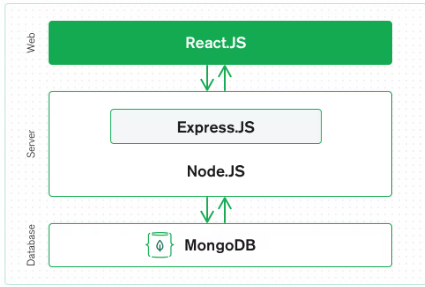
\includegraphics[width = 0.8\textwidth]{mernarchi.png}\\[0.1in]
    \caption{Architecture}
    \label{fig:my_label}
\end{figure}

\clearpage
\chapter{System Design}
\section{Data Flow Diagrams}

\subsection{Level 0 Data Flow Diagrams}
\begin{figure}[!htbp]
    \centering
    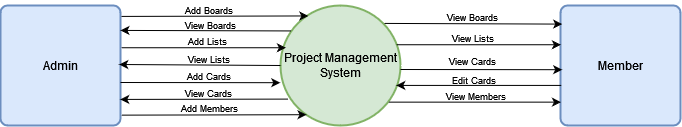
\includegraphics[scale = 0.6]{dataflow0.png}\\[0.1in]
    \caption{Level 0 DFD}
    \label{fig:my_label}
\end{figure}
\FloatBarrier


\subsection{Level 1 Data Flow Diagrams}
\begin{figure}[!htbp]
    \centering
    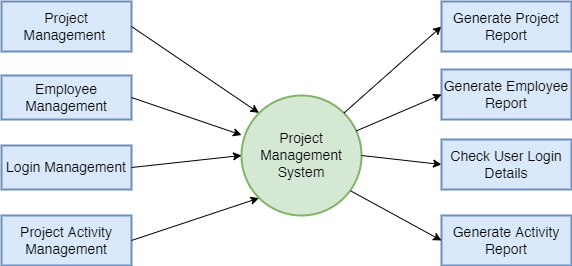
\includegraphics[scale = 0.6]{DFDlev1.drawio.png}\\[0.1in]
    \caption{Level 1 DFD}
    \label{fig:my_label}
\end{figure}
\FloatBarrier


\clearpage
\chapter{Detailed Design}
\section{UML Diagrams}

\subsection{Use Case Diagrams}
\begin{figure}[!htbp]
    \centering
    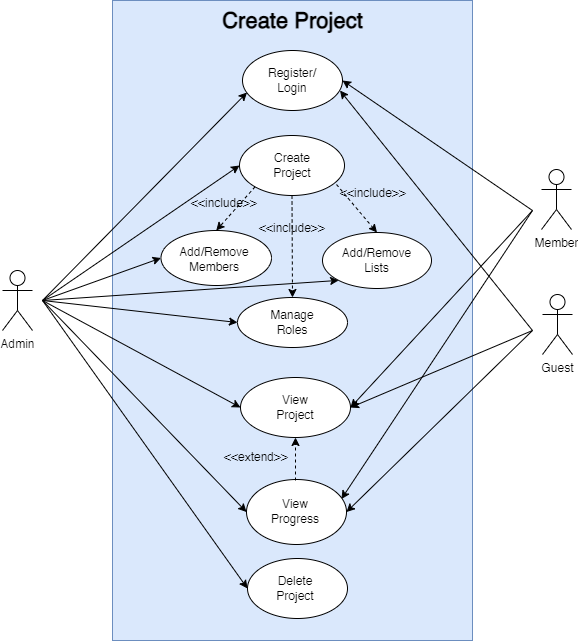
\includegraphics[width = 0.8\textwidth]{createproject.png}\\[0.1in]
    \caption{Create Project}
    \label{fig:my_label}
\end{figure}
The Actors are Admin, Member and Guest. Admin will do the functions like create/delete project, add/remove members to the project, manage roles etc. Member can login, view the project and view progress. The guest/client can view the project and it's progress.
\FloatBarrier

\begin{figure}[!htbp]
    \centering
    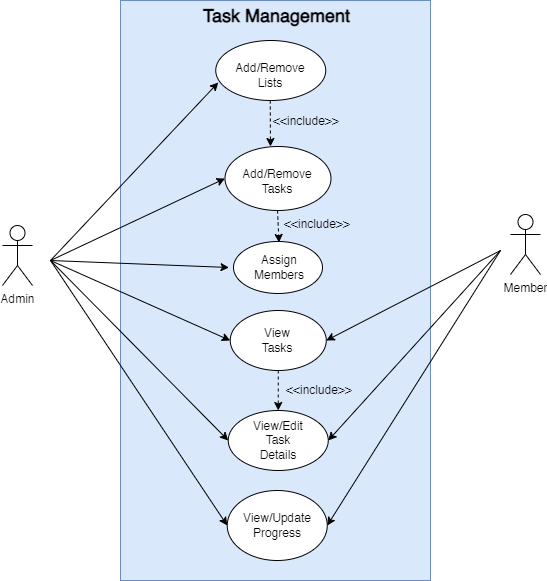
\includegraphics[width = 0.8\textwidth]{Tasksmngmnt.png}\\[0.1in]
    \caption{Task management}
    \label{fig:my_label}
\end{figure}

\FloatBarrier

\subsection{Class Diagrams}
\begin{figure}[!htbp]
    \centering
    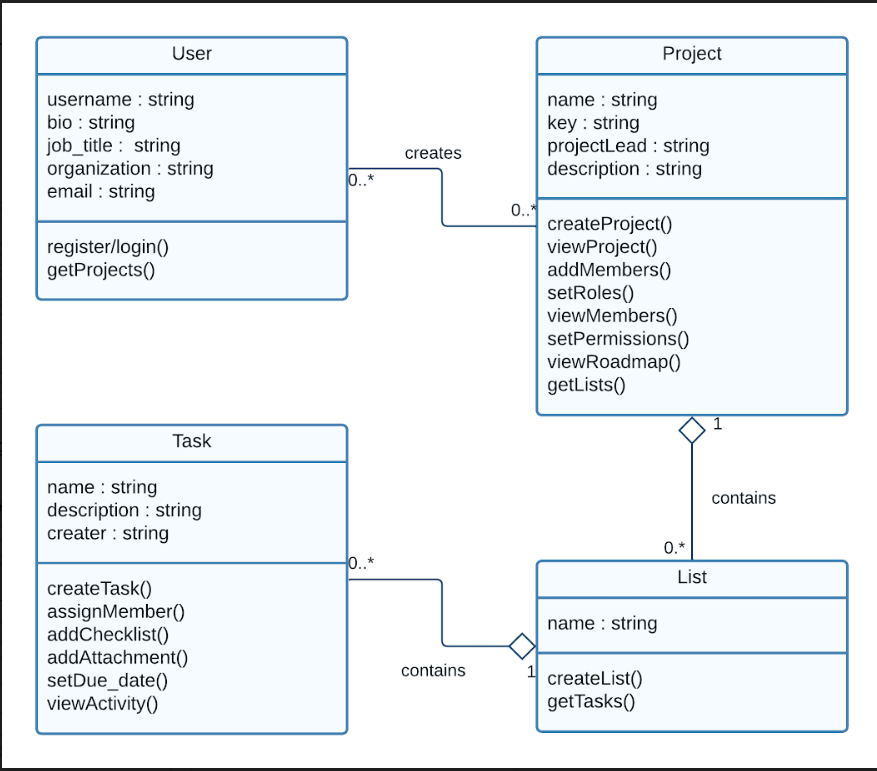
\includegraphics[width = 0.8\textwidth]{classdiagram.png}\\[0.1in]
    \caption{Class Diagram}
    \label{fig:my_label}
\end{figure}

\FloatBarrier
 
\subsection{Sequence Diagrams}

\begin{figure}[!htbp]
    \centering
    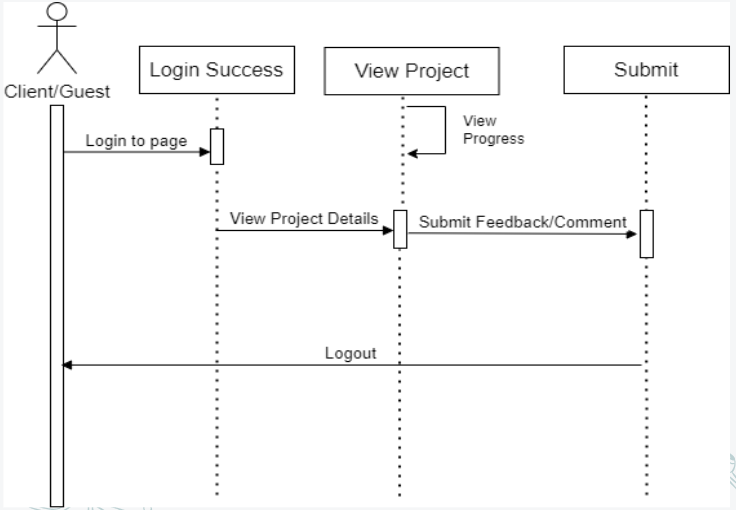
\includegraphics[width = 0.8\textwidth]{seqDgmClnt.png}\\[0.1in]
    \caption{Sequence Diagram for Client}
    \label{fig:my_label}
\end{figure}

\begin{figure}[h]
    \centering
    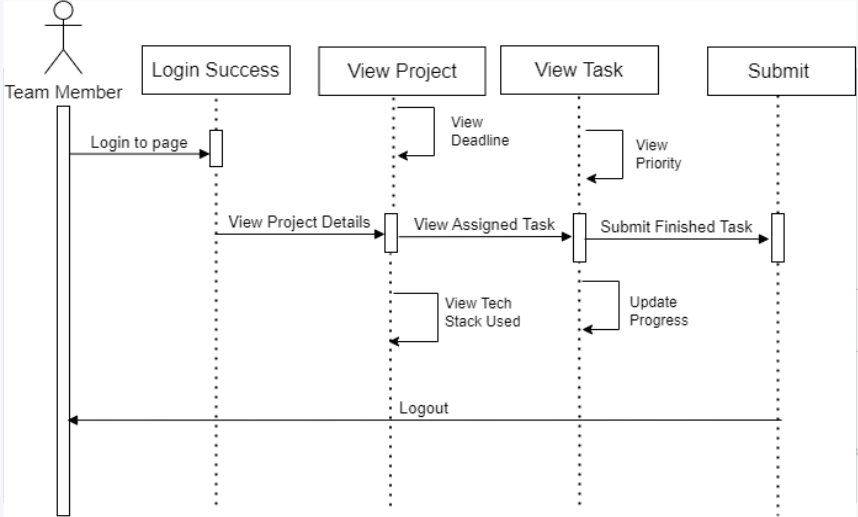
\includegraphics[width = 0.8\textwidth]{seqDiagramTeamMem.png}\\[0.1in]
    \caption{Sequence Diagram for Team members}
    \label{fig:my_label}
\end{figure}


\FloatBarrier

\subsection{Activity Diagrams}

\begin{figure}[!htbp]
    \centering
    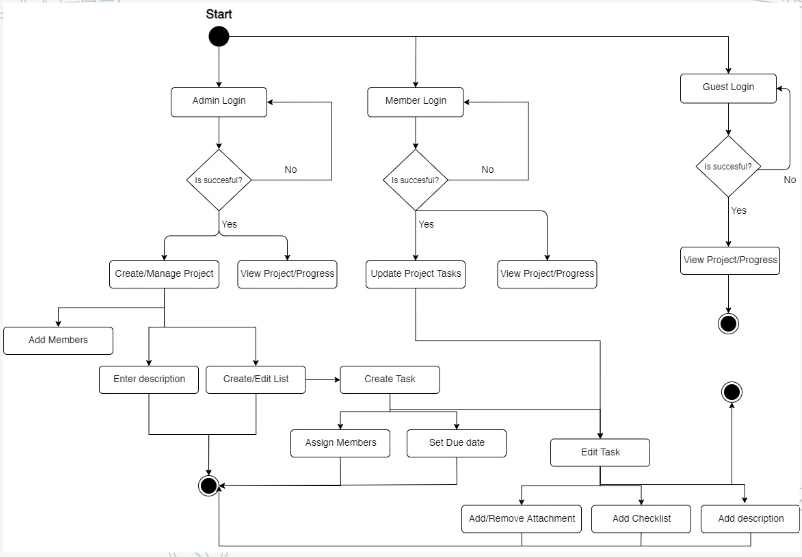
\includegraphics[width = 0.8\textwidth]{actvDgm.png}\\[0.1in]
    \caption{Activity Diagram}
    \label{fig:my_label}
\end{figure}




\chapter{Database Design}
\section{Data Dictionary}
\begin{table}[h]
\begin{tabular}[center]{|l|l|l|l|l|}
  \hline
  \multicolumn{5}{|c|}{User} \\
  \hline
  Fields & Data Type & Null/Not Null & Key & Default \\
  \hline
  name & varchar(50) & Not Null & - & - \\
  surnname & varchar(50) & Not Null & - & - \\
  email & varchar(50) & Not Null & PRI & - \\
  password & varchar(50) & Not Null & - & - \\
  avatar & varchar(50) & Not Null & - & - \\
  \hline
\end{tabular}
\caption{\label{tab:table-name}Data Dictionary for User.}
\end{table}

\vspace{10 mm}

\begin{table}[h]
\begin{tabular}[center]{|l|l|l|l|l|}
  \hline
  \multicolumn{5}{|c|}{Board} \\
  \hline
  Fields & Data Type & Null/Not Null & Key & Default \\
  \hline
  title & varchar(50) & Not Null & PRI & - \\
  members & varchar(50) & Not Null & - & - \\
  list & varchar(50) & Not Null & - & - \\
  activity & varchar(50) & Not Null & - & - \\
  isImage & boolean & Not Null & - & - \\
  background image link & varchar(50) & Not Null & - & - \\
  \hline
\end{tabular}
\caption{\label{tab:table-name}Data Dictionary for Board.}
\end{table}

\vspace{10 mm}

\begin{table}[h]
\begin{tabular}[center]{|l|l|l|l|l|}
  \hline
  \multicolumn{5}{|c|}{List} \\
  \hline
  Fields & Data Type & Null/Not Null & Key & Default \\
  \hline
  owner & varchar(50) & Not Null & - & - \\
  title & varchar(50) & Not Null & - & - \\
  \hline
\end{tabular}
\caption{\label{tab:table-name}Data Dictionary for List.}
\end{table}

\vspace{10 mm}

\begin{table}[h]
\begin{tabular}[center]{|l|l|l|l|l|}
  \hline
  \multicolumn{5}{|c|}{Card} \\
  \hline
  Fields & Data Type & Null/Not Null & Key & Default \\
  \hline
  name & varchar(50) & Not Null & - & - \\
  title & varchar(50) & Not Null & - & - \\
  checklist & varchar(50) & Not Null & - & - \\
  description & varchar(50) & Not Null & - & - \\
  labels & varchar(50) & Not Null & - & - \\
  %members & varchar(50) & Not Null & - & - \\
  date & date & Not Null & - & - \\
  attachments & varchar(50) & Not Null & - & - \\
  activities & varchar(50) & Not Null & - & - \\
  %owner & varchar(50) & Not Null & - & - \\
  %cover & varchar(50) & Not Null & - & - \\
  \hline
\end{tabular}
\caption{\label{tab:table-name}Data Dictionary for Card.}
\end{table}
\vspace{10 mm}

\section{ER Diagrams}
\begin{figure}[h]
    \centering
    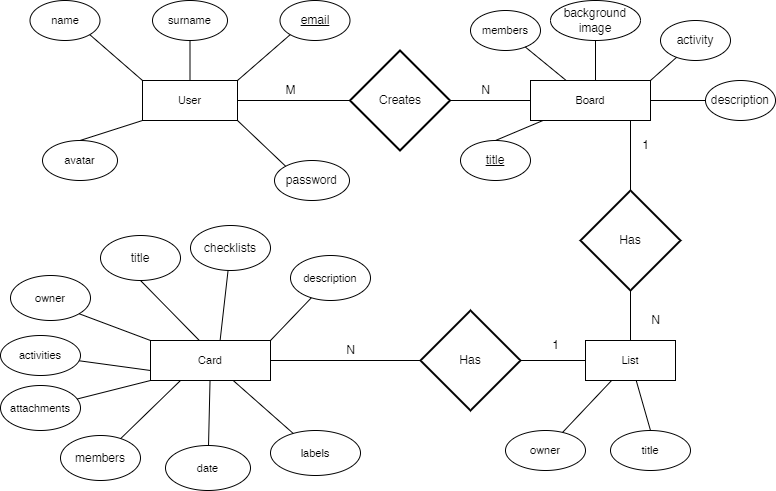
\includegraphics[width = 1.1\textwidth]{ER Diagram.drawio.png}\\[0.1in]
    \caption{ER Diagram}
    \label{fig:my_label}
\end{figure}
Include ER diagrams here and explain them
briefly




\chapter{Implementation details}
\section{System Requirements}
\subsection{Hardware requirements}
Processor: Intel core i3 or equivalent and higher\\
Installed Memory: 4.00 GB or higher
\subsection{Software requirements}
Operating System: Windows 10 or higher\\
Database: MongoDB\\
Web Technologies: HTML, CSS, JavaScript, React, NodeJS, ExpressJS\\
Text Editor:VS Code


\section{User Module}
\begin{figure}[!htbp]
    \centering
    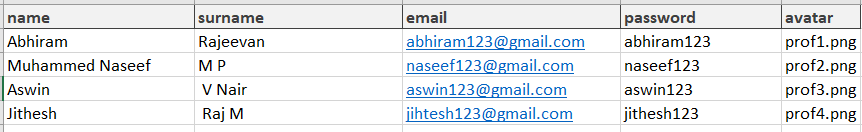
\includegraphics[scale = 0.6]{user.png}\\[0.1in]
    \caption{User Module}
    \label{fig:my_label}
\end{figure}
\FloatBarrier
\section{Board Module}
\begin{figure}[!htbp]
    \centering
    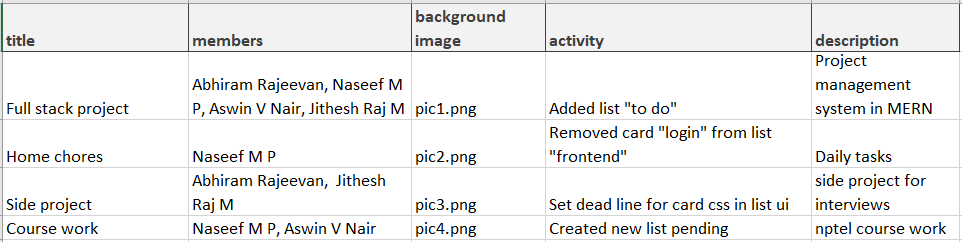
\includegraphics[scale = 0.6]{boards.png}\\[0.1in]
    \caption{Board Module}
    \label{fig:my_label}
\end{figure}
\FloatBarrier
\section{List Module}
\begin{figure}[!htbp]
    \centering
    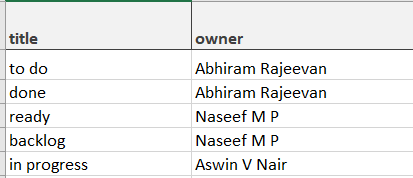
\includegraphics[scale = 0.6]{lists.png}\\[0.1in]
    \caption{List Module}
    \label{fig:my_label}
\end{figure}
\FloatBarrier
\section{Card Module}
\begin{figure}[!htbp]
    \centering
    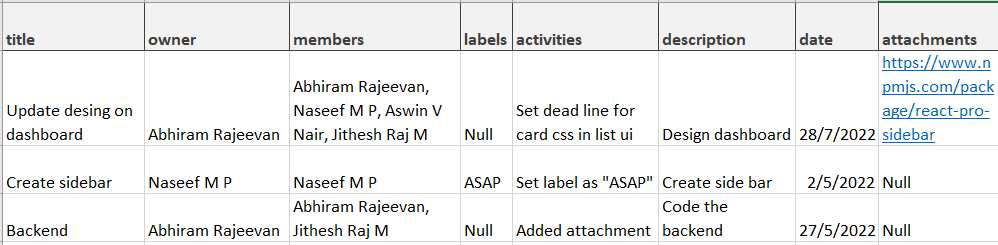
\includegraphics[scale = 0.6]{cards.png}\\[0.1in]
    \caption{Card Module}
    \label{fig:my_label}
\end{figure}
\FloatBarrier

% \chapter{Implementation details}
% \section{System Requirements}
% \subsection{Hardware requirements}

% \begin{itemize}
% \item {Processor:Intel(R) Core or higher}

%   \item {Installed Memory:4.00GB or higher}
%   \item {Speed:1.40GHz or faster}

%   \item {Operating System:32/64-Bit operating system, x86/x64-based processor}
%   \end{itemize}

% \subsection{Software requirements}
% \begin{itemize}
% \item {Operating System:Windows 7/8/8.1/10/11}

%   \item {Database:MongoDB}
%   \item {Web Server:Go}

%   \item {Web Technologies:HTML, CSS, JavaScript, and React}
%   \item {Text Editor:VS Code, VIM.}
%   \end{itemize}


% \section{User Components}
% \begin{itemize}
% \item {Registration/login}

%   \item {Search Item}
%   \item {view item}

%   \item {Add item}
%   \item {item details}
%   \item {Account}
%     \item {Subscription packages}
%   \end{itemize}





%\chapter{Experimental Results}
\begin{figure}[h]
\begin{subfigure}{.5\textwidth}
  \centering
  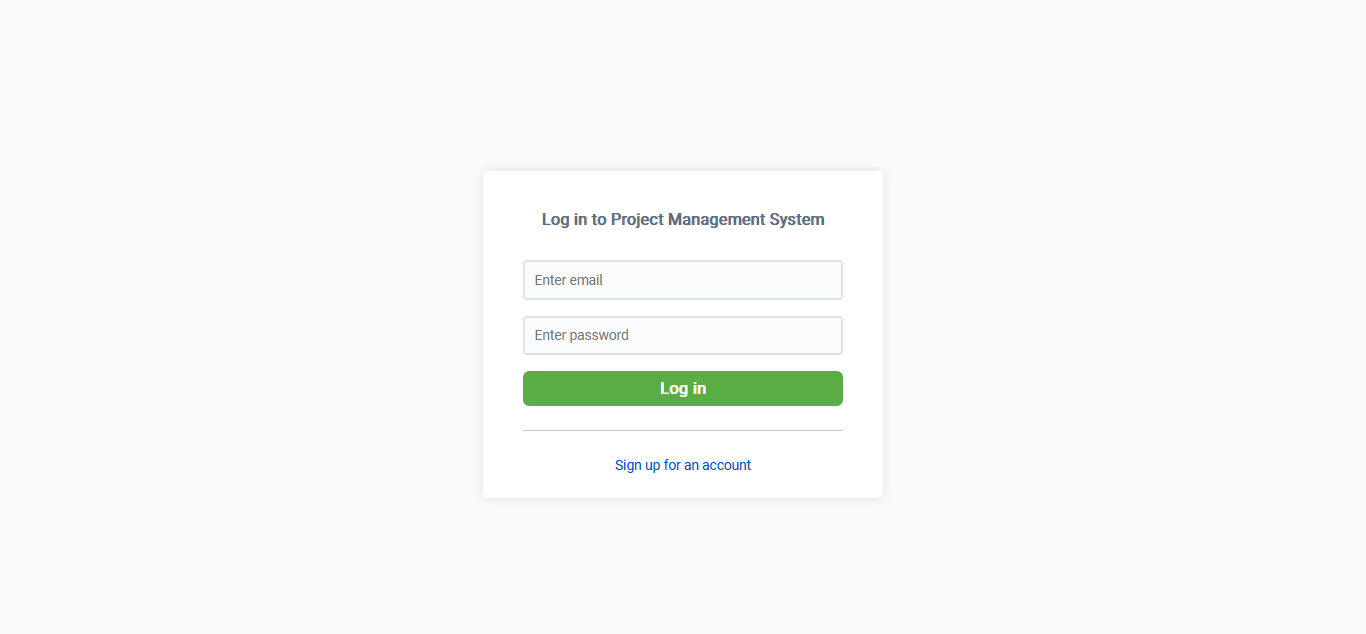
\includegraphics[width=2\linewidth]{login.png}
  \caption{Login page}
  \label{fig:sfig1}
\end{subfigure}%
\\
\begin{subfigure}{.5\textwidth}
  \centering
  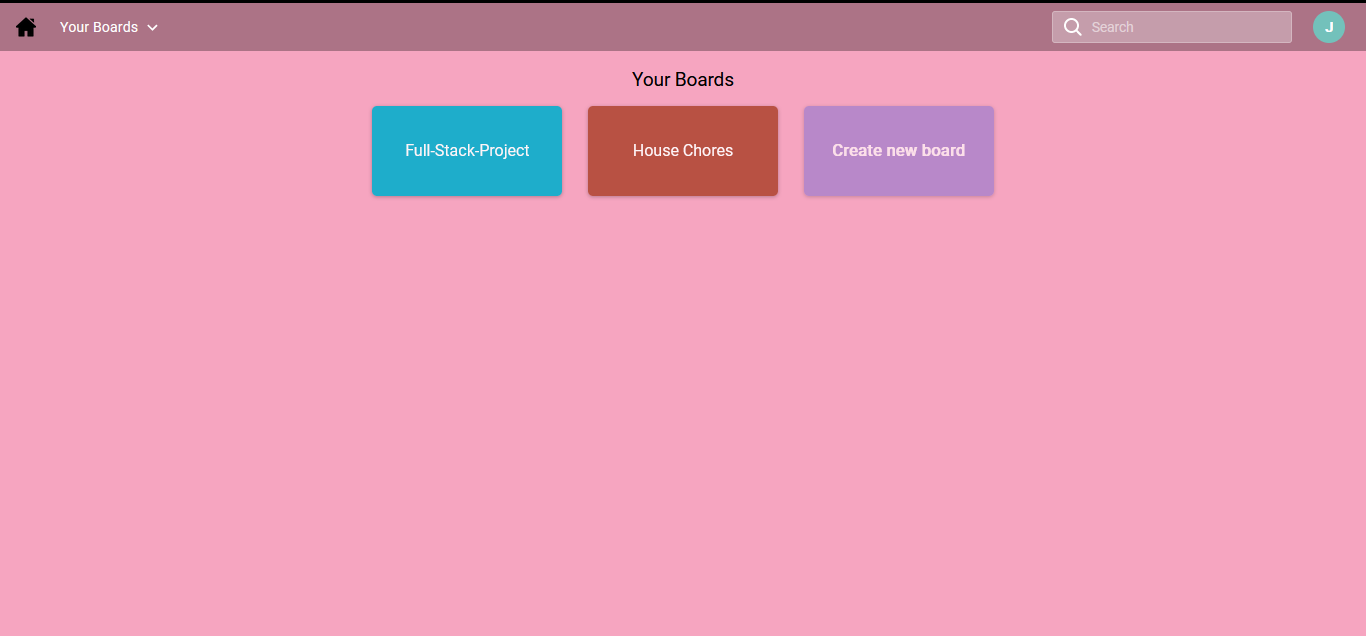
\includegraphics[width=2\linewidth]{boardspage.png}
  \caption{Boards page}
  \label{fig:sfig2}
\end{subfigure}
\\
\begin{subfigure}{.5\textwidth}
  \centering
  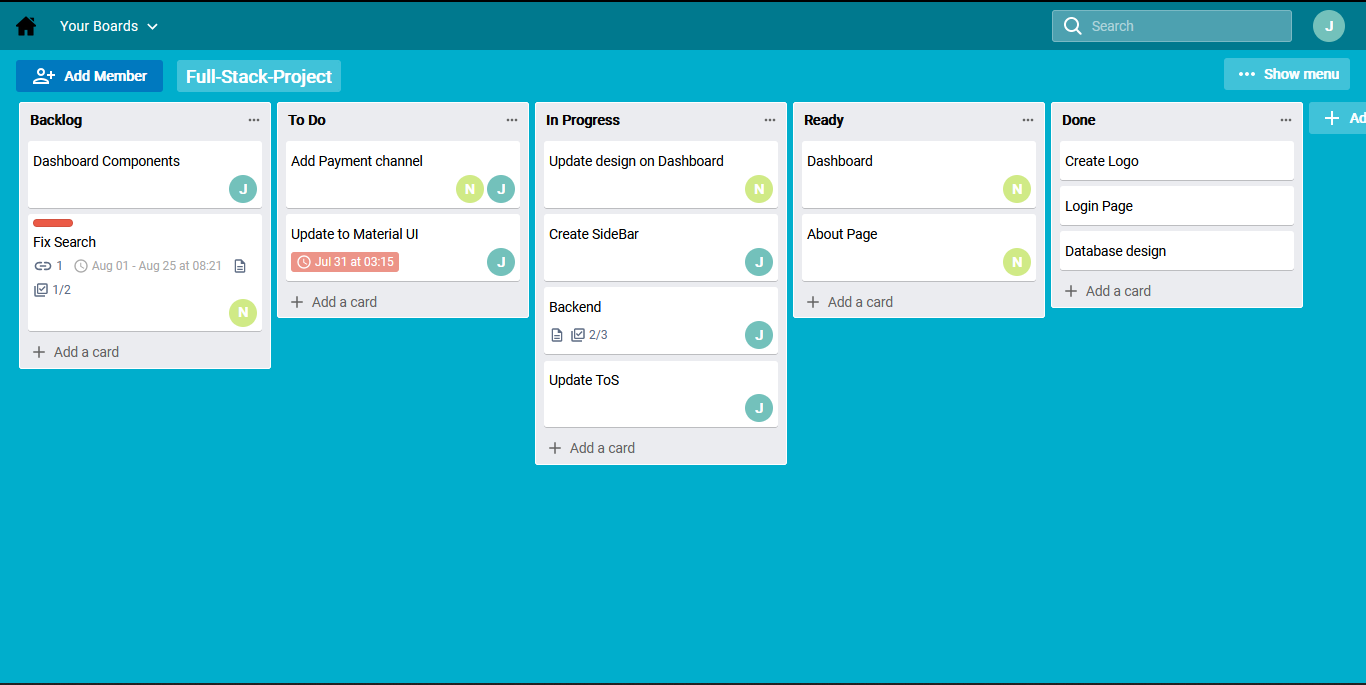
\includegraphics[width=2\linewidth]{boardpage.png}
  \caption{Board page}
  \label{fig:sfig1}
\end{subfigure}%
\end{figure}

\begin{figure}[h]
\ContinuedFloat
\begin{subfigure}{.5\textwidth}
  \centering
  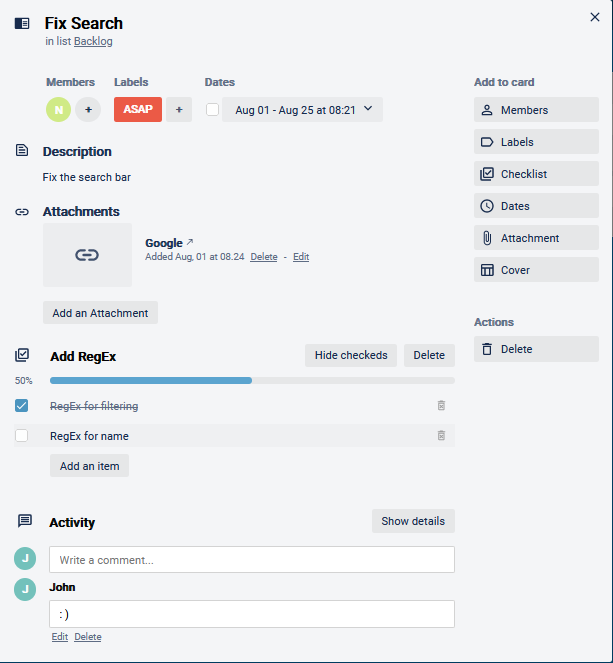
\includegraphics[width=2\linewidth]{taskeditor.png}
  \caption{Task editor}
  \label{fig:sfig1}
\end{subfigure}%
\caption{Web app demo}
\label{fig:fig}
\end{figure}
\chapter{Conclusions and Future Work}
The project management system was implemented successfully. This is a web app that helps in effective tracking of progress and management of tasks for projects. It is an open source solution to paid services available online that helps in project management. 

\printbibliography[heading=bibintoc]
\end{document}
